\documentclass[10pt, compress]{beamer}

\usetheme{m}

\usepackage{booktabs}
\usepackage[scale=2]{ccicons}
\usepackage{minted}

\usemintedstyle{trac}

\title{Eclipse Foundation}
\subtitle{A Non-Profit Open Source Corporation for the Eclipse IDE}
\date{\today}
\author{Alexandria Mack - Andrew Mandula - Katie Tigue}
\institute{}

\begin{document}

\maketitle

\section{What is it?}

\begin{frame}{What is it?}

\includegraphics[width=\textwidth]{images/EclipseLogo.jpg}
\begin{center}A Non-Profit Corporation to support the development of the Eclipse IDE, and other software \end{center}
\end{frame}
    
    \begin{frame}{What is it?}
    \textbf{Company}
    \begin{itemize}
    \item Company: Eclipse Foundation
    \item Founded: November 2001
    \item Restructured: February 2004
    \item HQ: Ottowa, Ontario, Canada
    \item Original Founders are No Longer Active
    \item 19 Employees
    \end{itemize}
    \end{frame}
    
\begin{frame}{What is it?}
\textbf{How it's Organized}
\begin{itemize}
\item Governe  d by a Board of Directors that includes both developers and consumers.
\item A full time support staff but does not employee the actual developers.
\item Funded by annual membership fees.
\end{itemize}
\end{frame}

\begin{frame}{What is it?}
\textbf{How to Contribute}
\begin{itemize}
\item Report/Fix a Bug
\item Commit to an Existing Project
\item Start a New Project
\end{itemize}
\end{frame}


\section{Communications}

\begin{frame}{Communications}

\textbf{Community}
\begin{itemize}
\item IRC Channel: \#eclipse irc.freenode.net
\item \href{http://git.eclipse.org/gitroot/platform/eclipse.platform.common.git master}{\alert{Self Hosted Repo}}
\item \href{http://www.eclipse.org/documentation/}{\alert{Documentation}}
\item \href{http://www.eclipse.org/forums/index.php?t=thread&frm_id=100 }{\alert{Forums}}
\end{itemize}

\end{frame}

\begin{frame}{Communications}

\textbf{Social Media}
\begin{itemize}
\item \href{https://twitter.com/EclipseFdn}{\alert{Twitter: 11.9K Followers}}
\item \href{https://www.facebook.com/eclipse.org }{\alert{Facebook: 79,478 Likes}}
\item \href{https://www.linkedin.com/company/eclipse-foundation}{\alert{Linkedin: 1,589 Followers}}
\item \href{https://plus.google.com/+Eclipse/}{\alert{Google+: 32,165 Followers}}
\item \href{https://www.youtube.com/user/EclipseFdn}{\alert{Youtube: 5,938 Subscribers}}
\end{itemize}

\end{frame}

\begin{frame}{Communications}

\textbf{Conferences}
\begin{itemize}
\item EclipseCon
\item \href{http://events.eclipse.org/}{\alert{Hackathons}}
\end{itemize}


\end{frame}

\section{Eclipse IDE}

\begin{frame}{Eclipse IDE}
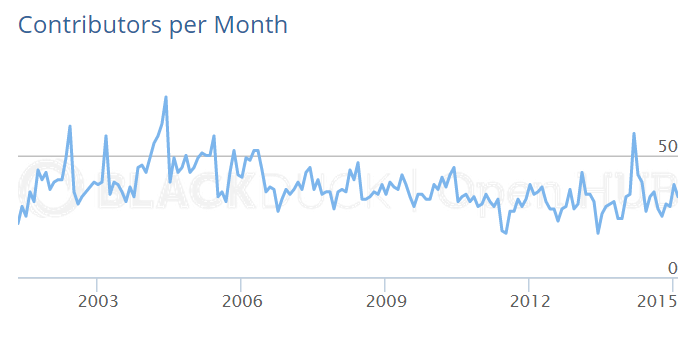
\includegraphics[width=\textwidth]{images/EclipseContributors.png}
    \begin{itemize}
    \item Initial Commit: 2003
    \item Latest Release: June 2013
    \item Founding Member: Mike Wilson
    \end{itemize}
\end{frame}

\begin{frame}{Eclipse IDE}
    \textbf{\href{http://www.eclipse.org/legal/epl-v10.html}{Eclipse Public License}}
    \begin{itemize}
    \item all projects adhere to it
    \item "non-exclusive, worldwide, royalty-free patent license under Licensed Patents to make, use, sell, offer to sell, import and otherwise transfer the Contribution"
    \end{itemize}
\end{frame}

\begin{frame}{Summary}

  Get the source of this theme and the demo presentation from

  \begin{center}\url{github.com/matze/mtheme}\end{center}

  The theme \emph{itself} is licensed under a
  \href{http://creativecommons.org/licenses/by-sa/4.0/}{Creative Commons
  Attribution-ShareAlike 4.0 International License}.

  \begin{center}\ccbysa\end{center}

\end{frame}

\plain{}{Questions?}

\end{document}
